\renewcommand{\chaptername}{Capitulo}
\chapter{Anexo I: Manual de instalación del Módulo RDF de DSpace 6.2 en Windows 10} 
\section{Introducción}

La plataforma DSpace 6.2 contiene un módulo RDF, sin embargo, es necesario instalar un servicio aparte para poderlo hacer funcionar. En ese sentido, la documentación de DSpace sugiere instalar Apache Jena Fuseki\footnote{Disponible en \textit{https://jena.apache.org/download/index.cgi}}, que es un servidor EndPoint para realizar consultas en lenguaje SPARQL, y que también ofrece el servicio \textit{Triple Store} o almacén de ternas.\newline

\begin{figure}[!ht]
	\centering
	\fbox{
	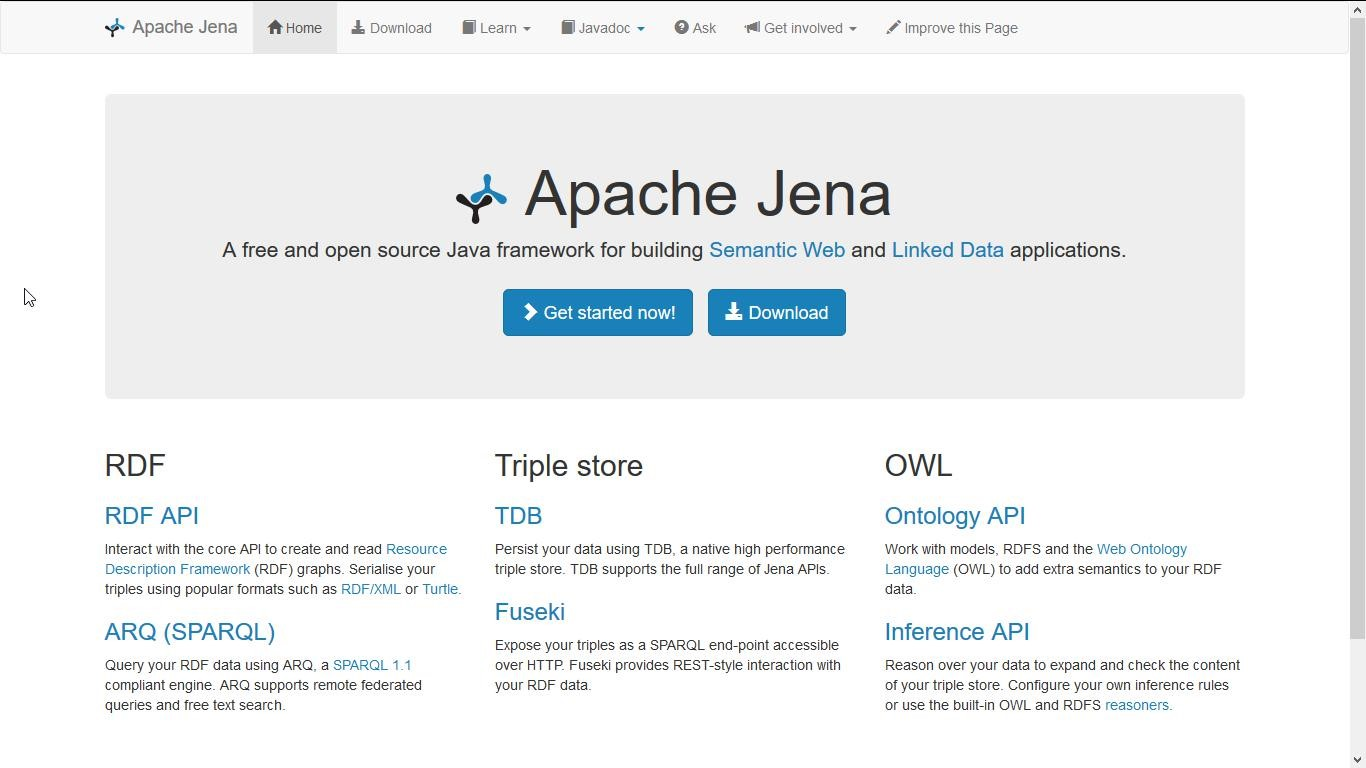
\includegraphics[width=14cm]{figures/Anexo/Site_Apache_Jena.jpg}} 
    \caption{Página principal del Apache Jena Fuseki}
    \label{landing-page-apache-jena-fiseki}
\end{figure}

Características del equipo de cómputo para la instalación de Jena Fuseki:

\begin{itemize}
    \item Sistema operativo Windows 10 de 64 bits
    \item 4Gb de Memoria RAM mínima recomendable
    \item 50Gb de espacio en disco duro mínimo recomendable
    \item DSpace 6.2 previamente instalado
\end{itemize}{}

\section{Descarga de Apache Jena Fuseki 1.6}

Usando cualquier navegador web de su elección (preferentemente Chrome versión 76 o Mozilla versión 68, para 64 bits) se accede a la dirección \textit{http://archive.apache.org/dist/jena/binaries/jena-fuseki1-1.6.0-distribution.zip} para descargar la carpeta comprimida que se muestra en la Figura \ref{ventana-descarga-apache-jena-fiseki}. Una vez que se muestra la ventana de descarga, se presiona la opción “Guardar” y después la opción “Aceptar”. Verifique la carpeta “Descargas” (se puede seleccionar otra ubicación del archivo si se desea) para ubicar el archivo \textit{jena-fuseki1-1.6.0-distribution.zip} que contiene los archivos de instalación de Jena-Fuseki.

\begin{figure}[!ht]
	\centering
	\fbox{
	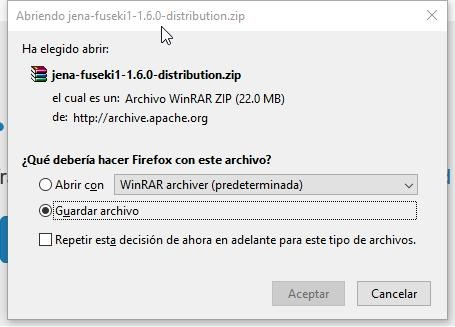
\includegraphics[width=12cm]{figures/Anexo/Ventaja_descarga.jpg}} 
    \caption{Ventana de descarga de Apache Jena Fuseki}
    \label{ventana-descarga-apache-jena-fiseki}
\end{figure}

La carpeta descargada contiene los archivos necesarios para realizar la instalación del servidor Jena-Fuseki en el mismo servidor de DSpace 6.2. Se puede emplear winrar, winzip o el servicio de descompresión de Windows para acceder al contenido de la carpeta, el cual se muestra en la Figura \ref{ventana-contenido-apache-jena-fiseki}.

\begin{figure}[!ht]
	\centering
	\fbox{
	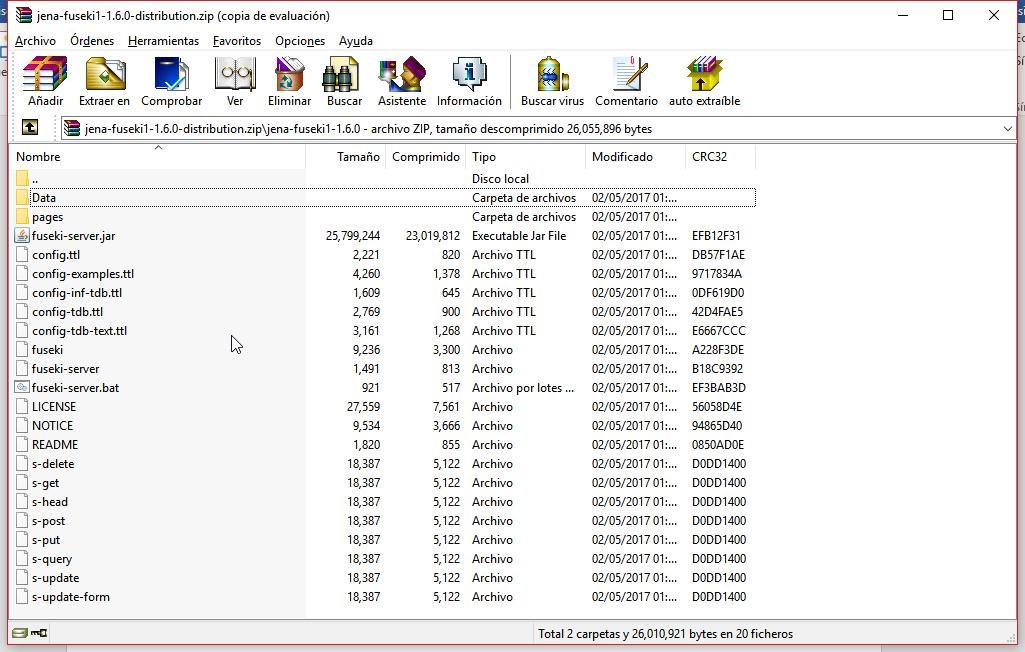
\includegraphics[width=12cm]{figures/Anexo/Contenido_carpeta.jpg}} 
    \caption{Contenido de la carpeta comprimida descargada}
    \label{ventana-contenido-apache-jena-fiseki}
\end{figure}

\section{Instalación}

Para instalar el servidor de Jena-Fuseki se crea una nueva carpeta en el disco duro C con el nombre de "Jena". Una vez creada la carpeta "Jena" de descomprime es esa ubicación el contenido de la carpeta comprimida \textit{jena-fuseki1-1.6.0-distribution.zip}, como se muestra en la Figura \ref{contenido-carpeta-apache-jena-fiseki}.

\begin{figure}[!ht]
	\centering
	\fbox{
	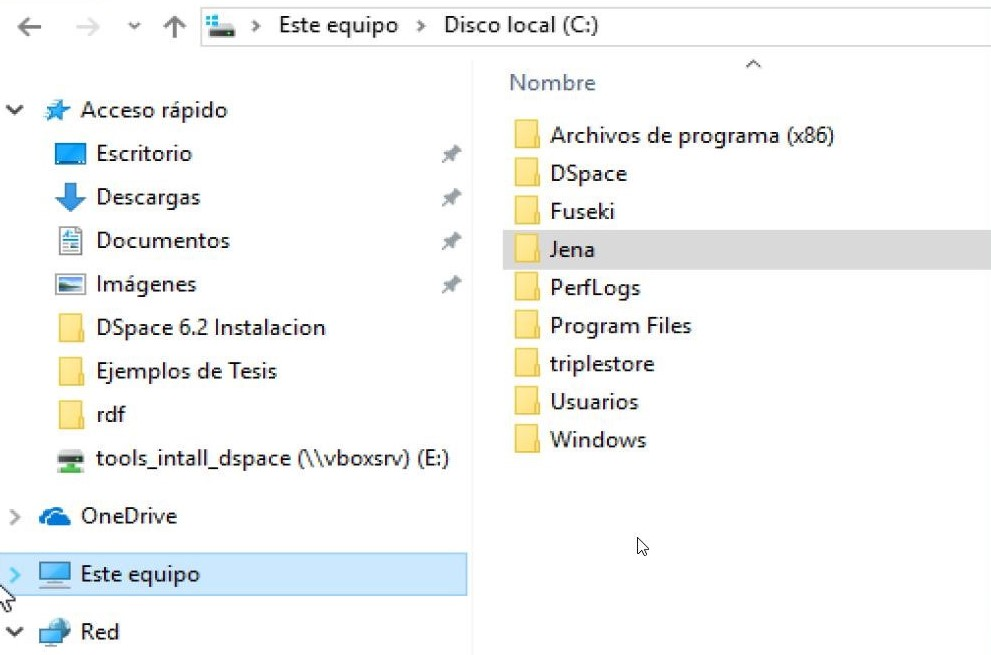
\includegraphics[width=12cm]{figures/Anexo/Instalacion.jpg}} 
    \caption{Contenido de la carpeta comprimida descargada}
    \label{contenido-carpeta-apache-jena-fiseki}
\end{figure}

La Figura \ref{contenido-instalacion-apache-jena-fiseki} muestra el contenido de la carpeta \textit{Jena} creada en el disco C.

\begin{figure}[!ht]
	\centering
	\fbox{
	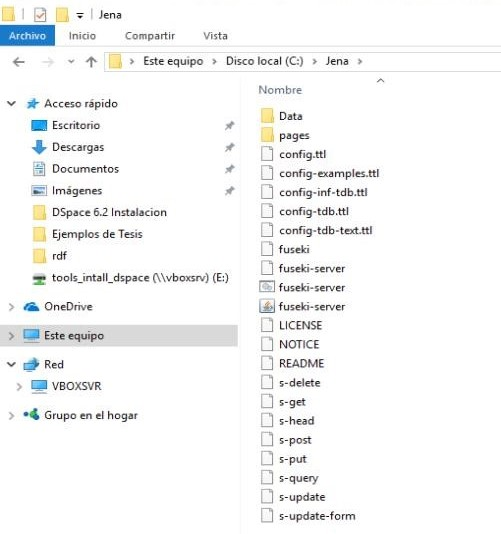
\includegraphics[width=12cm]{figures/Anexo/Contenido_instalacion.jpg}} 
    \caption{Contenido de la carpeta comprimida descargada}
    \label{contenido-instalacion-apache-jena-fiseki}
\end{figure}

\section{Configuración}

De manera similar que en la instalación, es necesario crear una nueva carpeta en el disco C y nombrarla "triplestore", como lo muestra la Figura \ref{carpeta-triplestore-apache-jena-fiseki}.\newline

\begin{figure}[!ht]
	\centering
	\fbox{
	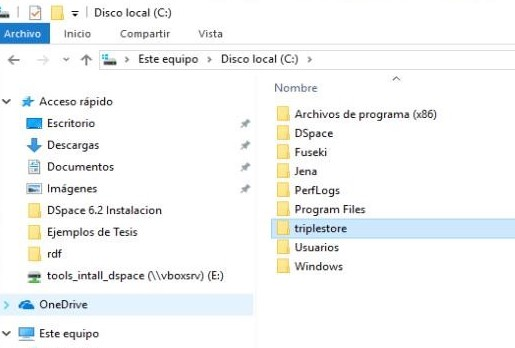
\includegraphics[width=12cm]{figures/Anexo/Carpeta_TripleStore.jpg}} 
    \caption{Creación de la carpeta \textit{triplestore}}
    \label{carpeta-triplestore-apache-jena-fiseki}
\end{figure}

Posteriormente, se requiere editar el archivo \textit{fuseki-assembler.ttl} ubicado en la ruta \textit{c:\DSpace\config\modules\rdf} como se muestra en la Figura \ref{configuracion-apache-jena-fiseki}. Antes de editar se sugiere realizar una copia del archivo para restaurar la configuración original en caso de fallo. Para editar el archivo puede emplear notepad, notepad++ o cualquier otro editor de textos.\newline

\begin{figure}[!ht]
	\centering
	\fbox{
	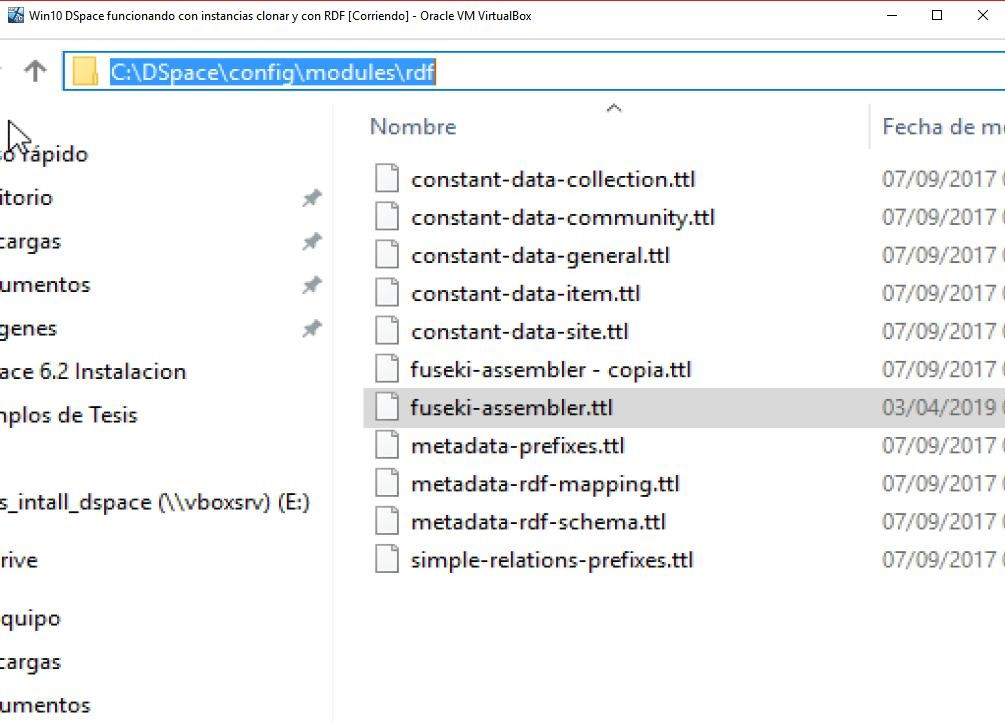
\includegraphics[width=12cm]{figures/Anexo/Configuracion_fuseki.jpg}} 
    \caption{Creación de la carpeta \textit{triplestore}}
    \label{configuracion-apache-jena-fiseki}
\end{figure}

Dentro del archivo \textit{fuseki-assembler.ttl} es necesario colocar la ubicación del almacén de ternas (carpeta triplestore) en la ruta \textit{tdb:location 'c:/triplestore'} como se muestra en la Figura \ref{configuracion-serializador-jena-fiseki}.

\begin{figure}[!ht]
	\centering
	\fbox{
	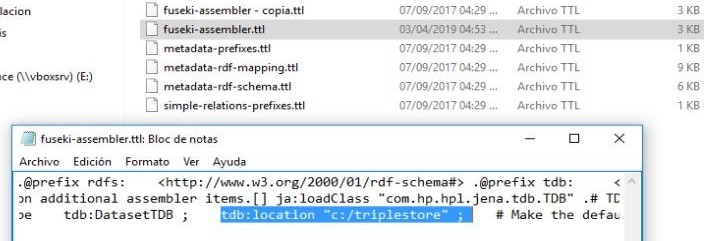
\includegraphics[width=12cm]{figures/Anexo/Parametro_configuracion.jpg}} 
    \caption{Configuración del serializador \textit{fiseki-assembler.ttl}}
    \label{configuracion-serializador-jena-fiseki}
\end{figure}

\section{Arranque de Apache Jena Fuseki}

Para arrancar el servidor hay que entrar a la carpeta \textit{c:/Jena} y ejecutar el comando \textit{ fuseki-server.bat –localhost –config=c:\dspace\config\modules\rdf\fuseki-assembler.ttl} y espere el mensaje \textit{Started <fecha actual> CST on port 3030} como se muestra en la Figura \ref{ejecucion-serializador-jena-fiseki}.

\begin{figure}[!ht]
	\centering
	\fbox{
	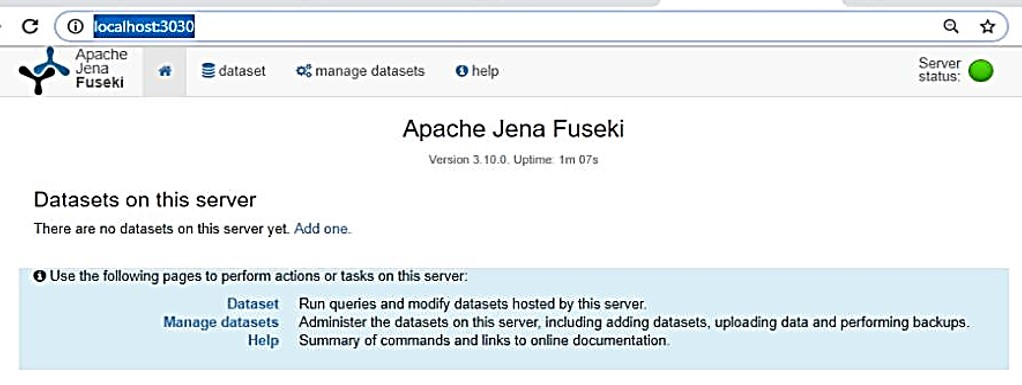
\includegraphics[width=12cm]{figures/ejecuccionJenaFuseki.jpg}} 
    \caption{Ejecución de Apache Jena Fiseki}
    \label{ejecucion-jena-fiseki}
\end{figure}

Para verificar que el servicio se esta ejecutando correctamente, se puede abrir un navegador como Google Chrome o Mozilla Firefox y se introduce la dirección \textit{http://localhost:3030} y \textit{http://localhost:3030/sparql.tpl} para acceder al servicio de consultas usando el lenguaje SPARQL, como se muestra en la Figura \ref{ejecucion-jena-fiseki-query}.

\begin{figure}[!ht]
	\centering
	\fbox{
	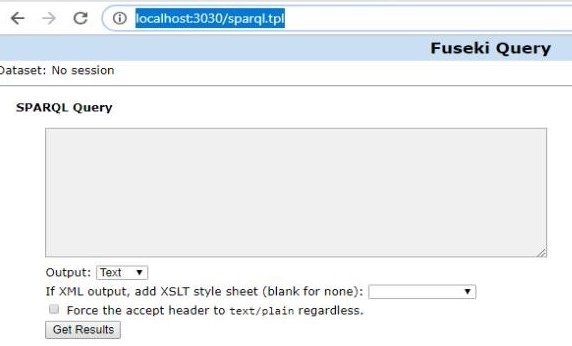
\includegraphics[width=12cm]{figures/Anexo/Fuseki_query.jpg}} 
    \caption{Ejecución del servicio Fuseki Query}
    \label{ejecucion-jena-fiseki-query}
\end{figure}

\section{Arranque del módulo RDF de DSpace 6.2}

Antes de poder ejecutar el módulo RDF de DSpace es necesario ejecutar el serializador que realice la migración de los metadatos almacenados en DSpace hacia el almacén de ternas. Para arrancar el serializador es necesario abrir una consola del sistema (Inicio + r para abrir la ventana ejecutar, escribir cmd y presionar enter o ejecutar). Se accede a la ruta \textit{c:/DSpace/bin} y se ejecuta el comando \textit{dspace rdfizer –convert-all} como se muestra en la figura \ref{ejecucion-serializador-jena-fiseki}.

\begin{figure}[!ht]
	\centering
	\fbox{
	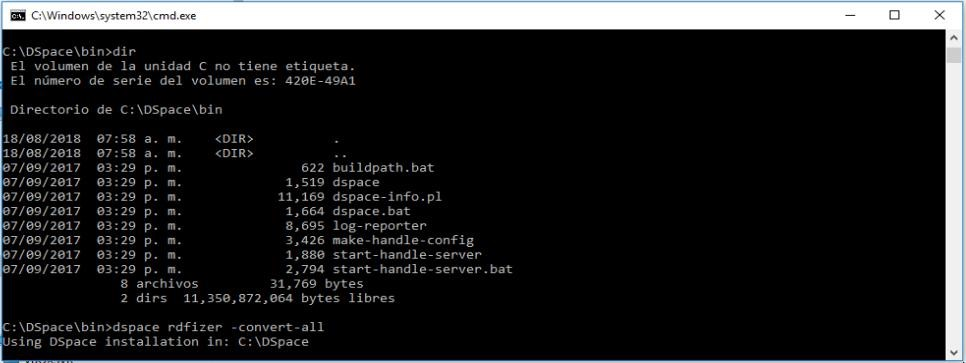
\includegraphics[width=12cm]{figures/Anexo/Serializacion.jpg}} 
    \caption{Ejecución del serializador \textit{fiseki-assembler.ttl}}
    \label{ejecucion-serializador-jena-fiseki}
\end{figure}

\section{Acceso a servicio RDF a través de interfaz web}

Finalmente, para verificar que el servicio RDF está funcionando, se debe acceder a cualquiera de los ítems agregados e introducir la URL de la siguiente manera: sustituir \textit{/xmlui/} por \textit{/rdf/} y al final de la URL agregar \textit{http://localhost:8080/xmlui/handle/123456789/36} sustituir por \textit{http://localhost:8080/rdf/handle/123456789/ttl} como se muestra en las Figuras \ref{acceso-item-dspace} a Y.

\begin{figure}[!ht]
	\centering
	\fbox{
	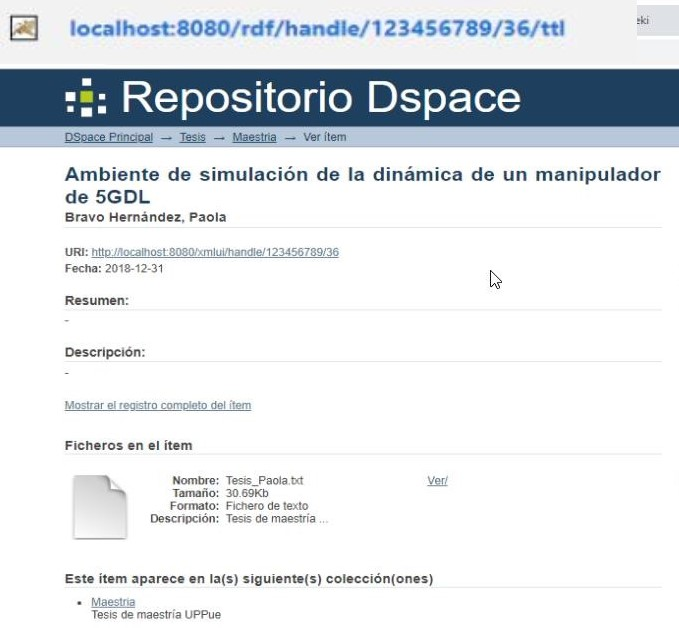
\includegraphics[width=12cm]{figures/Anexo/item_dspace.jpg}} 
    \caption{Acceso a ítem de DSpace mediante URL}
    \label{acceso-item-dspace}
\end{figure}

\begin{figure}[!ht]
	\centering
	\fbox{
	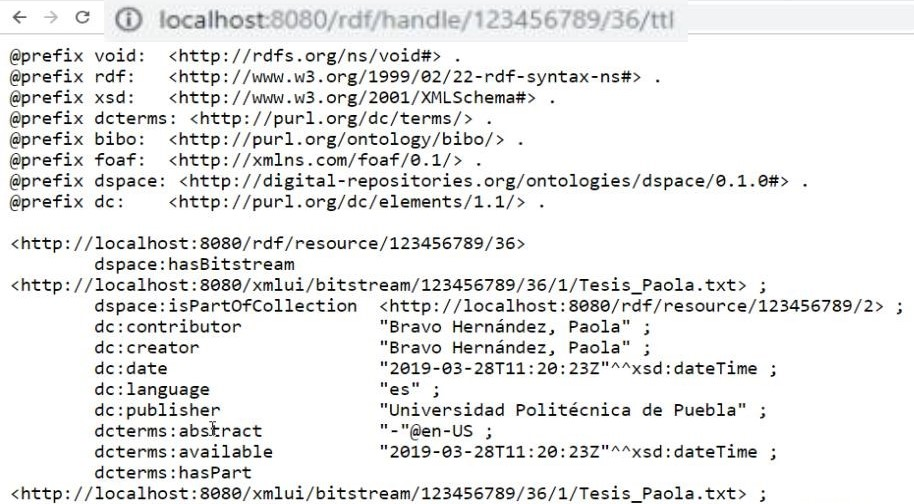
\includegraphics[width=12cm]{figures/Anexo/Documento_RDF.jpg}} 
    \caption{Acceso a documento RDF migrado al almacén de ternas a través de una URL}
    \label{acceso-rdf-dspace}
\end{figure}